\section{Istruzioni per l'uso}
\label{istruzioni}

Il presente capitolo offre una visione e una guida al corretto utilizzo delle principali funzionalità disponibili agli utenti.\\
Sono presenti le seguenti sezioni:

\begin{itemize}
\item  \hyperref[autenticazione]{Autenticazione};
\item  \hyperref[registrazione]{Registrazione};
\item  \hyperref[home]{Navigazione nella pagina principale};
\item  \hyperref[userdata]{Gestione delle credenziali};
\item  \hyperref[iscrizione]{Iscrizione ad un processo};
\item  \hyperref[gestione]{Esecuzione di un processo};
\item  \hyperref[logout]{Chiusura della sessione}.
\end{itemize}

\pagebreak

\subsection{Autenticazione}
\label{autenticazione}

In figura \hyperref[fig:Flogin]{figura \ref{fig:Flogin}}, è rappresentata la schermata iniziale del prodotto \progetto{}, in cui viene richiesto l'inserimento dello \textit{username} e della \textit{password} dell'utente.

\begin{figure}[H] \centering 
\frame{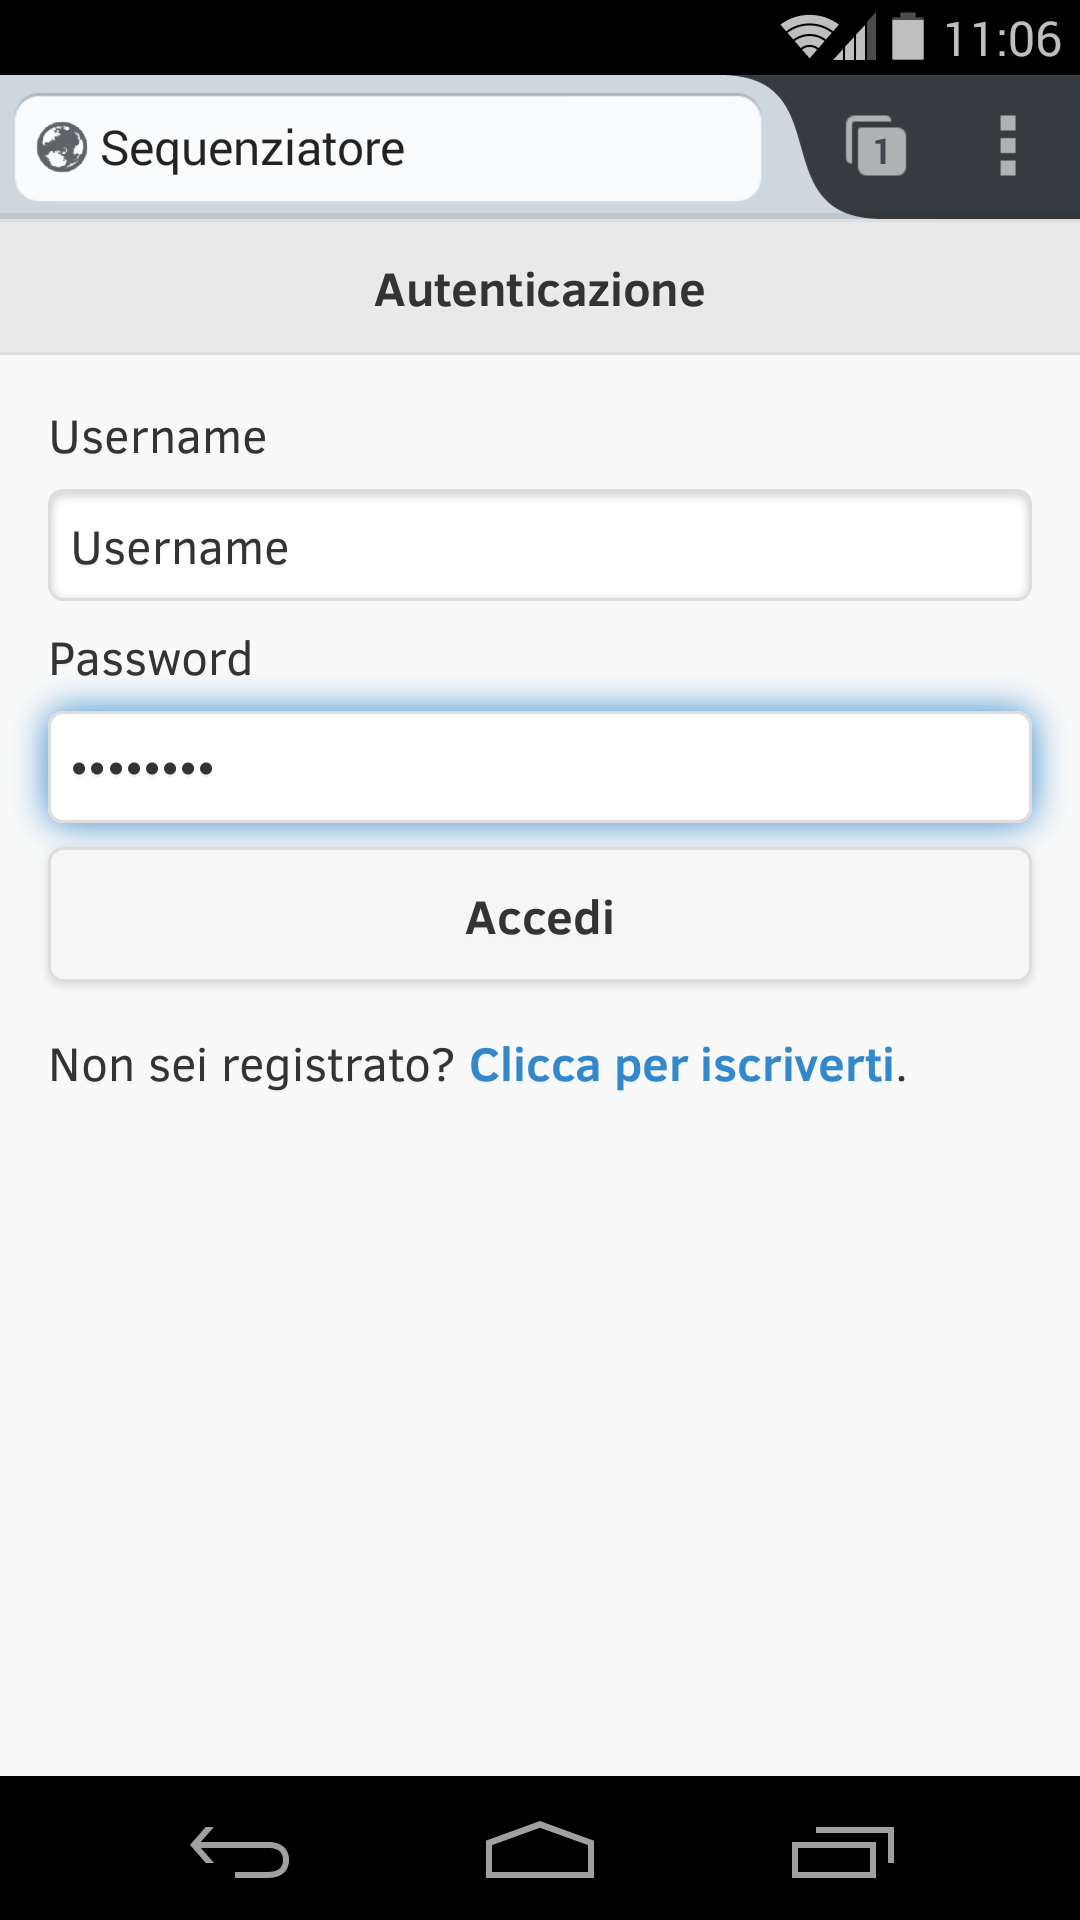
\includegraphics[width=0.5\textwidth]
{./screen/Login.png}} \caption{Schermata di autenticazione}
\label{fig:Flogin}
\end{figure}

Le credenziali di \textit{default} dell'utente sono quelle scelte in fase di \hyperref[Registrazione]{Registrazione}.
Se l'utente non è ancora registrato al sistema, può iscriversi premendo sul testo ``Clicca per iscriverti''.
Successivamente all'inserimento delle credenziali, è sufficiente selezionare il pulsante ``Accedi'', per accedere alle funzionalità dell'applicazione.

\subsubsection*{Possibili errori:}
\begin{itemize}
\item \hyperref[e1]{E1}: \textit{javascript\ped{G}} disabilitato;
\item \hyperref[e2]{E2}: credenziali non corrette;
\item \hyperref[e3]{E3}: errore di connessione al \textit{server\ped{G}}.
\end{itemize}

\subsection{Registrazione}
\label{registrazione}

\iffalse
In figura \hyperref[fig:Fregister]{figura \ref{fig:Fregister}}, è rappresentata la schermata di registrazione del prodotto \progetto{}, in cui viene richiesto l'inserimento dei dati dell'utente.

\begin{figure}[H] \centering 
\frame{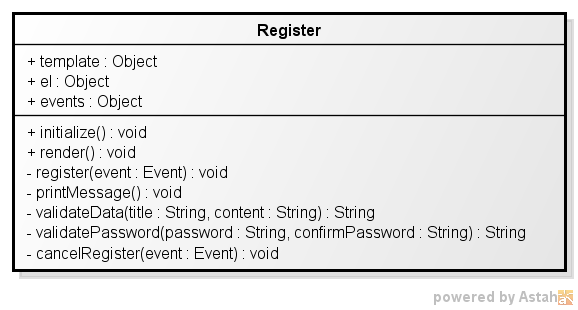
\includegraphics[width=0.5\textwidth]
{./screen/Register.png}} \caption{Schermata di registrazione}
\label{fig:Fregister}
\end{figure}
\fi

In questa pagina è possibile iscriversi al sistema \progetto{}.
Viene richiesto l'inserimento dei seguenti dati:
\begin{itemize}
\item \textbf{Nome:} nome dell'utente che vuole iscriversi;
\item \textbf{Cognome:} cognome dell'utente che vuole iscriversi;
\item \textbf{Username:} nome che verrà utilizzato per accedere al sistema;
\item \textbf{Password:} password che verrà utilizzata per accedere al sistema. Deve essere composta da almeno 8 caratteri;
\item \textbf{Email:} \textit{email} dell'utente che vuole iscriversi;
\item \textbf{Data di nascita:}data di nascita dell'utente che vuole iscriversi.
\end{itemize}

Per concludere la registrazione è sufficiente selezionare il pulsante ``Registrati''.

\subsubsection*{Possibili errori:}
\begin{itemize}
\item \hyperref[e1]{E1}: \textit{javascript\ped{G}} disabilitato;
\item \hyperref[e3]{E3}: errore di connessione al \textit{server\ped{G}};
\item \hyperref[e4]{E4}: \textit{username} già utilizzato;
\item \hyperref[e5]{E5}: dato mancante;
\item \hyperref[e6]{E6}: \textit{email} già utilizzata;
\item \hyperref[e7]{E7}: \textit{email} non valida;
\end{itemize}

\subsection{Navigazione nella pagina principale}
\label{home}
\iffalse
In figura \hyperref[fig:Fhome]{figura \ref{fig:Fhome}}, è rappresentata la schermata della \textit{homepage} del progetto \progetto{}, accessibile dopo aver effettuato l'autenticazione, che consente di scegliere una delle funzionalità di base disponibili.

\begin{figure}[H] \centering 
\frame{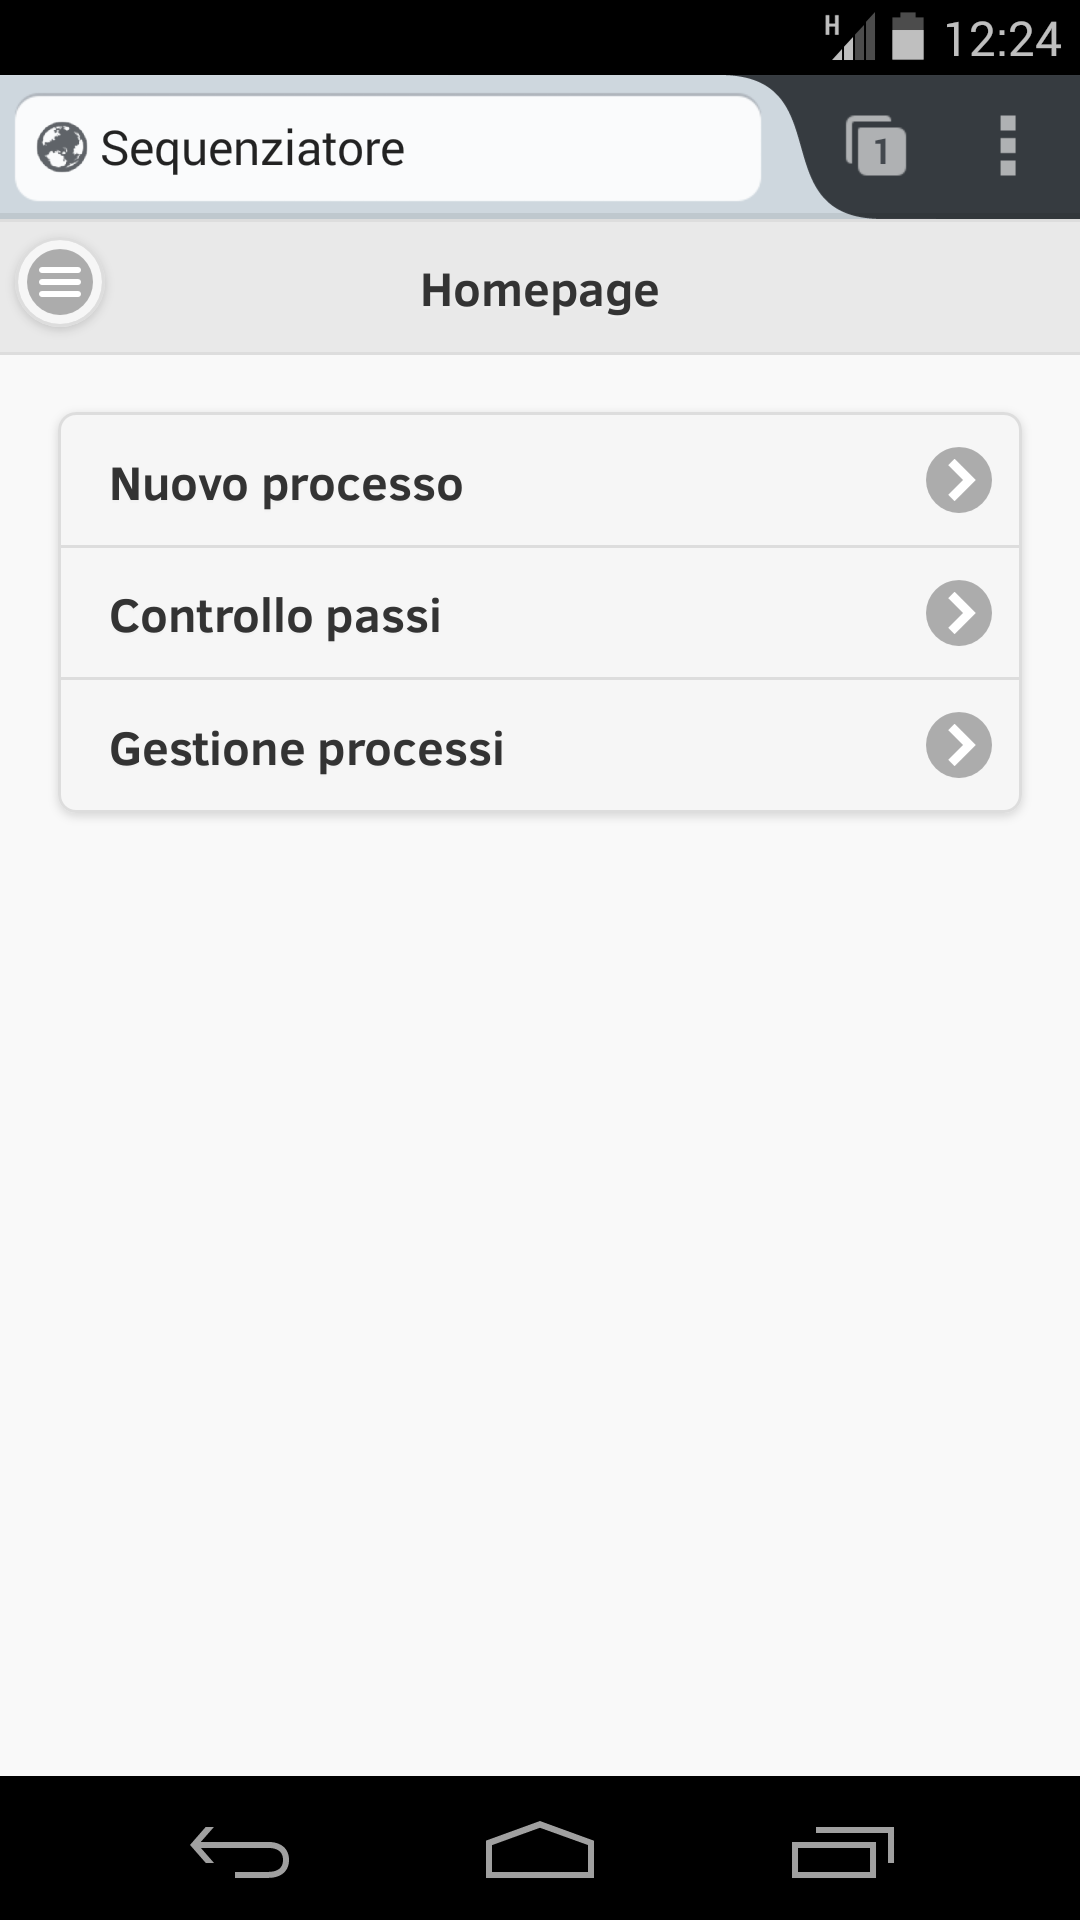
\includegraphics[width=0.5\textwidth]
{./screen/Home.png}} \caption{Homepage}
\label{fig:Fhome}
\end{figure}
\fi
In questa pagina è possibile selezionare uno dei seguenti pulsanti per iniziare la gestione delle rispettive funzionalità:
\begin{itemize}
\item  \hyperref[iscrizione]{Iscrizione ad un processo};
\item  \hyperref[gestione]{Esecuzione processi}.
\end{itemize}

Selezionando il pulsante in alto a sinistra, è possibile aprire il pannello laterale in cui è consentita la \hyperref[logout]{chiusura della sessione} e la \hyperref[userdata]{gestione delle credenziali}.

\subsubsection*{Possibili errori:}
\begin{itemize}
\item \hyperref[e1]{E1}: \textit{javascript\ped{G}} disabilitato.
\end{itemize}

\subsection{Gestione delle credenziali}
\label{userdata}

Per accedere alla funzionalità di gestione delle credenziali, è sufficiente aprire il pannello laterale rappresentato \hyperref[fig:Flogout]{figura \ref{fig:Flogout}}, accessibile per i soli utenti autenticati, e premere il pulsante ``Gestione credenziali''.

\begin{figure}[H] \centering 
\frame{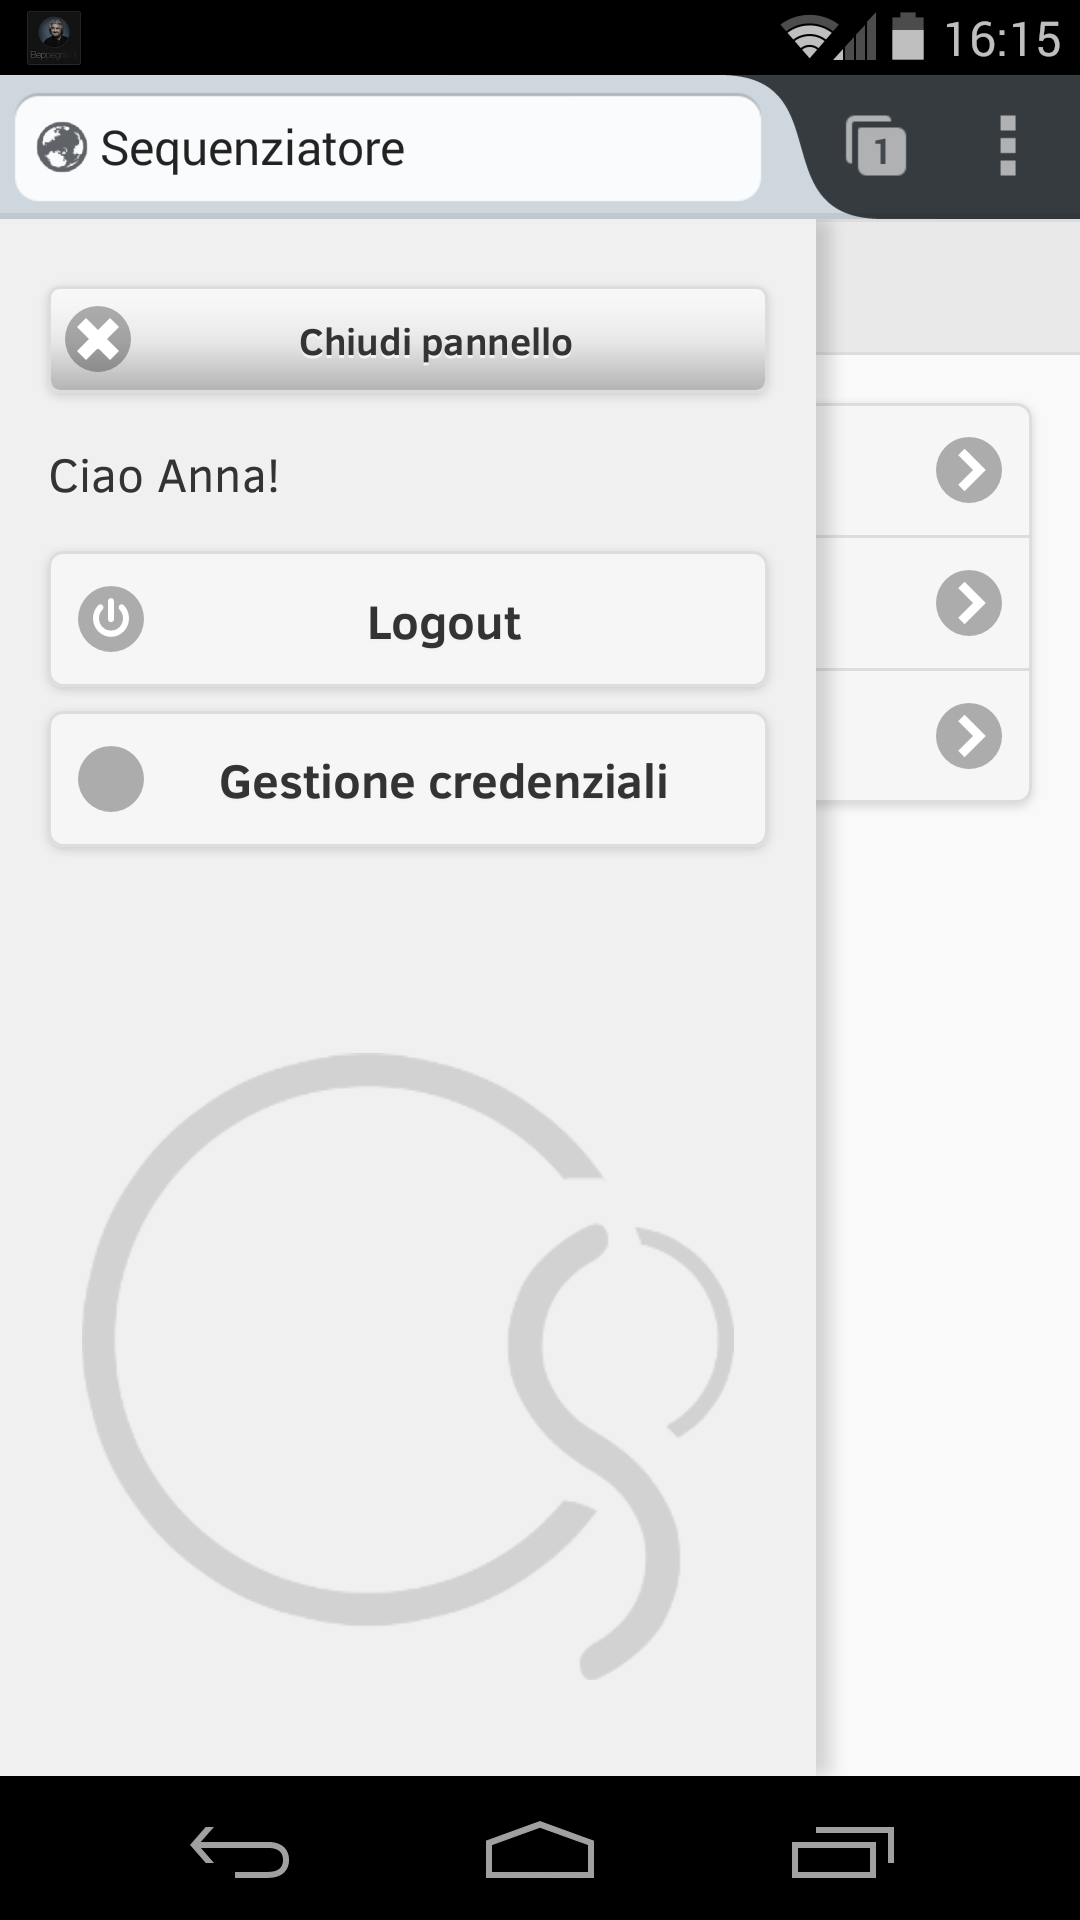
\includegraphics[width=0.5\textwidth]
{./screen/Logout.png}} \caption{Pannello laterale}
\label{fig:Flogout}
\end{figure}

\iffalse
In figura \hyperref[fig:Fregister]{figura \ref{fig:Fregister}}, è rappresentata la schermata di gestione delle credenziali utente.

\begin{figure}[H] \centering 
\frame{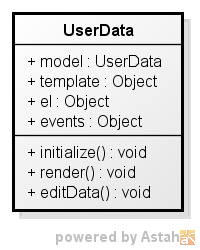
\includegraphics[width=0.5\textwidth]
{./screen/UserData.png}} \caption{Gestione delle credenziali}
\label{fig:Fuserdata}
\end{figure}
\fi

In questa pagina è possibile visualizzare e modificare le credenziali inserire in fase di registrazione.
È possibile modificare la propria \textit{email} e la propria \textit{password}.
Per favorire la sicurezza dell'applicazione, per modificare la \textit{password} è necessario inserire anche la \textit{password} corrente.

In altro a sinistra sono presenti i seguenti pulsanti:
\begin{itemize}
\item \textbf{Home:} pulsante che consente di tornare alla \hyperref[home]{pagina principale};
\item \textbf{Opzioni:} apre il pannello laterale in cui è consentita la \hyperref[logout]{chiusura della sessione}.
\end{itemize}

\subsubsection*{Possibili errori:}
\begin{itemize}
\item \hyperref[e1]{E1}: \textit{javascript\ped{G}} disabilitato;
\item \hyperref[e2]{E2}: credenziali non valide;
\item \hyperref[e3]{E3}: errore di connessione al \textit{server\ped{G}};
\item \hyperref[e6]{E6}: \textit{email} già utilizzata;
\item \hyperref[e7]{E7}: \textit{email} non valida.
\end{itemize}

\subsection{Iscrizione ad un processo}
\label{iscrizione}

\subsubsection{Scelta di un processo}

In figura \hyperref[fig:Fprocesses]{figura \ref{fig:Fprocesses}}, è rappresentata la schermata di gestione dei processia cui è possibili iscriversi, accessibile dopo aver effettuato l'autenticazione, che consente di selezionare un processo per gestirlo.

\begin{figure}[H] \centering 
\frame{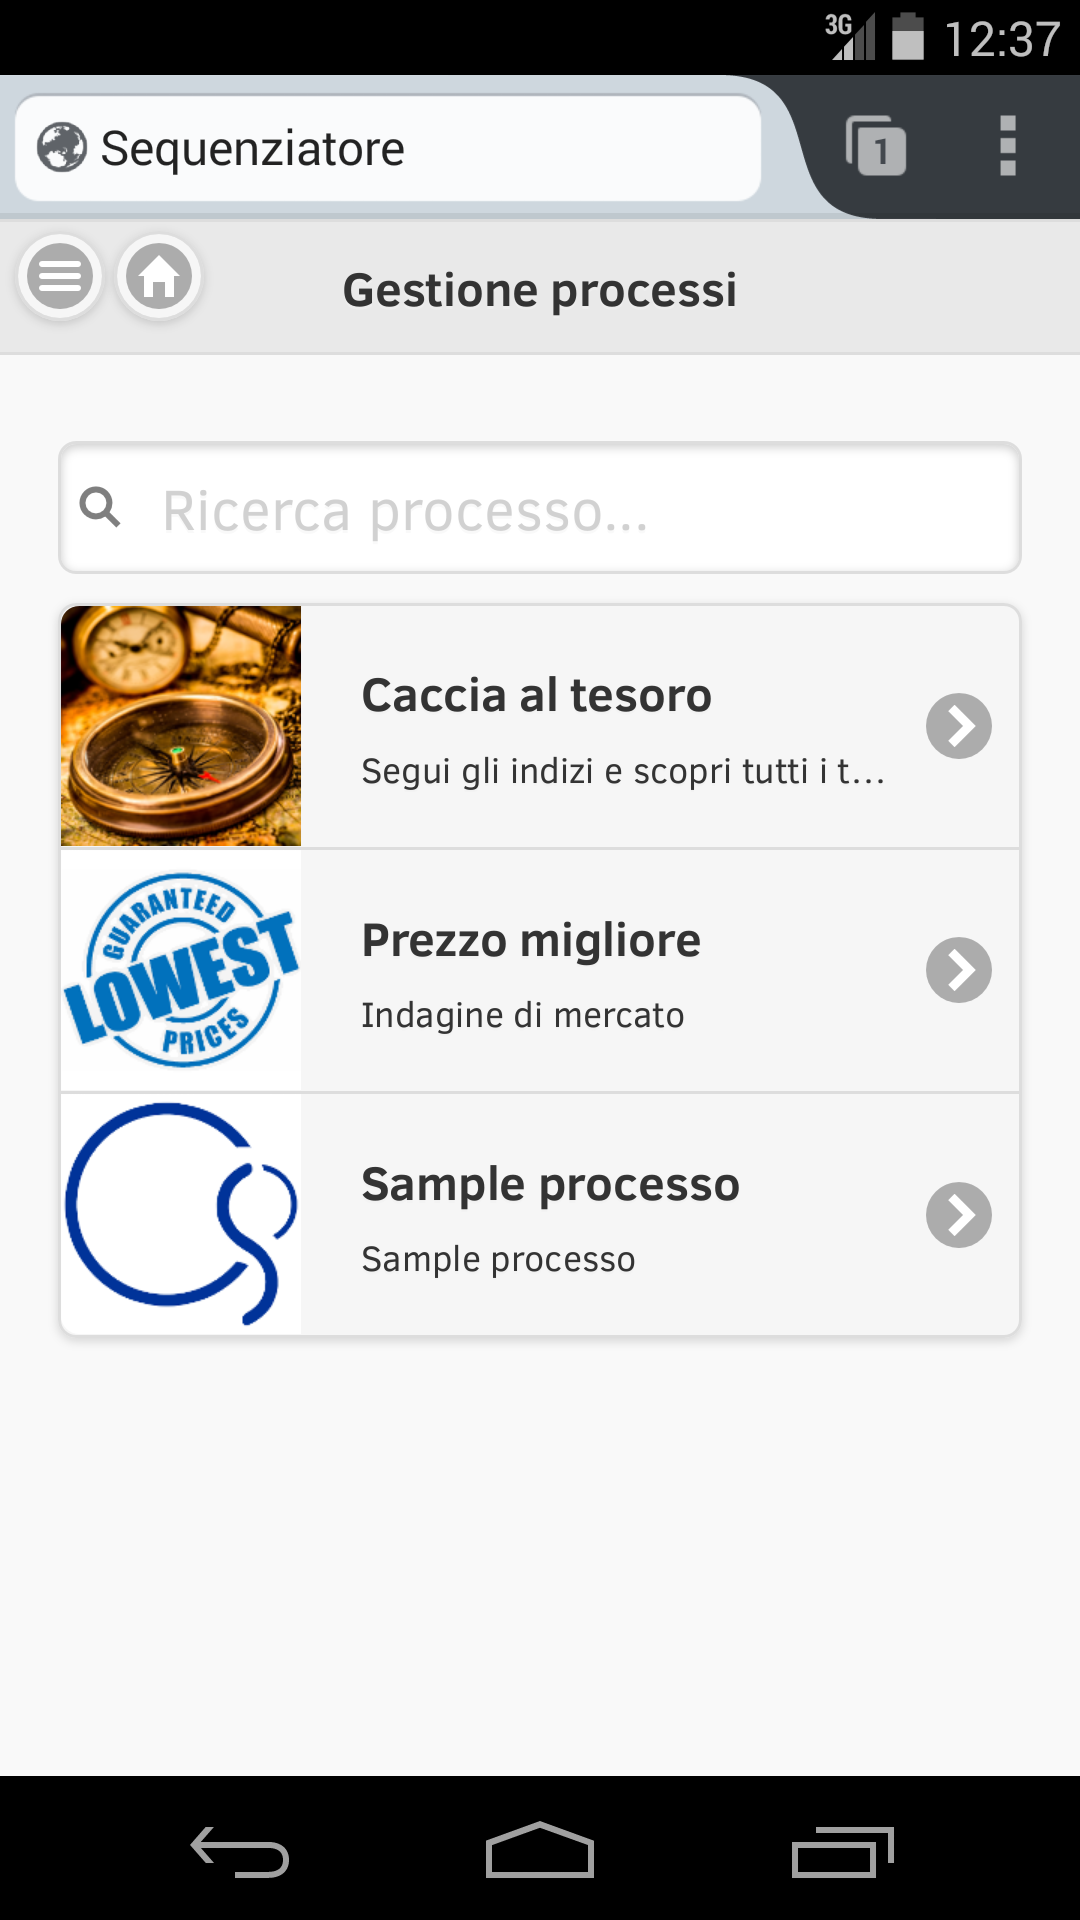
\includegraphics[width=0.5\textwidth]
{./screen/Processes.png}} \caption{Scelta di un processo}
\label{fig:Fprocesses}
\end{figure}

In questa pagina è possibile selezionare uno tra i processi in elenco. È inoltre disponibile la funzionalità di ricerca: inserendo del testo nella barra di ricerca (con suscritto ``Ricerca processo''), l'elenco si aggiornerà, con i soli processi che contengono nel titolo o nella descrizione, il testo oggetto della ricerca.
Per ripristinare l'elenco è sufficiente cancellare il testo nella barra dell'elenco, o premere il pulsante a forma di ``x''.

In altro a sinistra sono presenti i seguenti pulsanti:
\begin{itemize}
\item \textbf{Home:} pulsante che consente di tornare alla \hyperref[home]{pagina principale};
\item \textbf{Opzioni:} apre il pannello laterale in cui è consentita la \hyperref[logout]{chiusura della sessione} e la \hyperref[userdata]{gestione delle credenziali}.
\end{itemize}

\paragraph*{Possibili errori:}
\begin{itemize}
\item \hyperref[e1]{E1}: \textit{javascript\ped{G}} disabilitato;
\item \hyperref[e3]{E3}: errore di connessione al \textit{server\ped{G}}.
\end{itemize}

\subsubsection{Iscrizione al processo selezionato}
\iffalse
In figura \hyperref[fig:Fprocess]{figura \ref{fig:Fprocess}}, è rappresentata la schermata di gestione di un processo al quale è possibile iscriversi.

\begin{figure}[H] \centering 
\frame{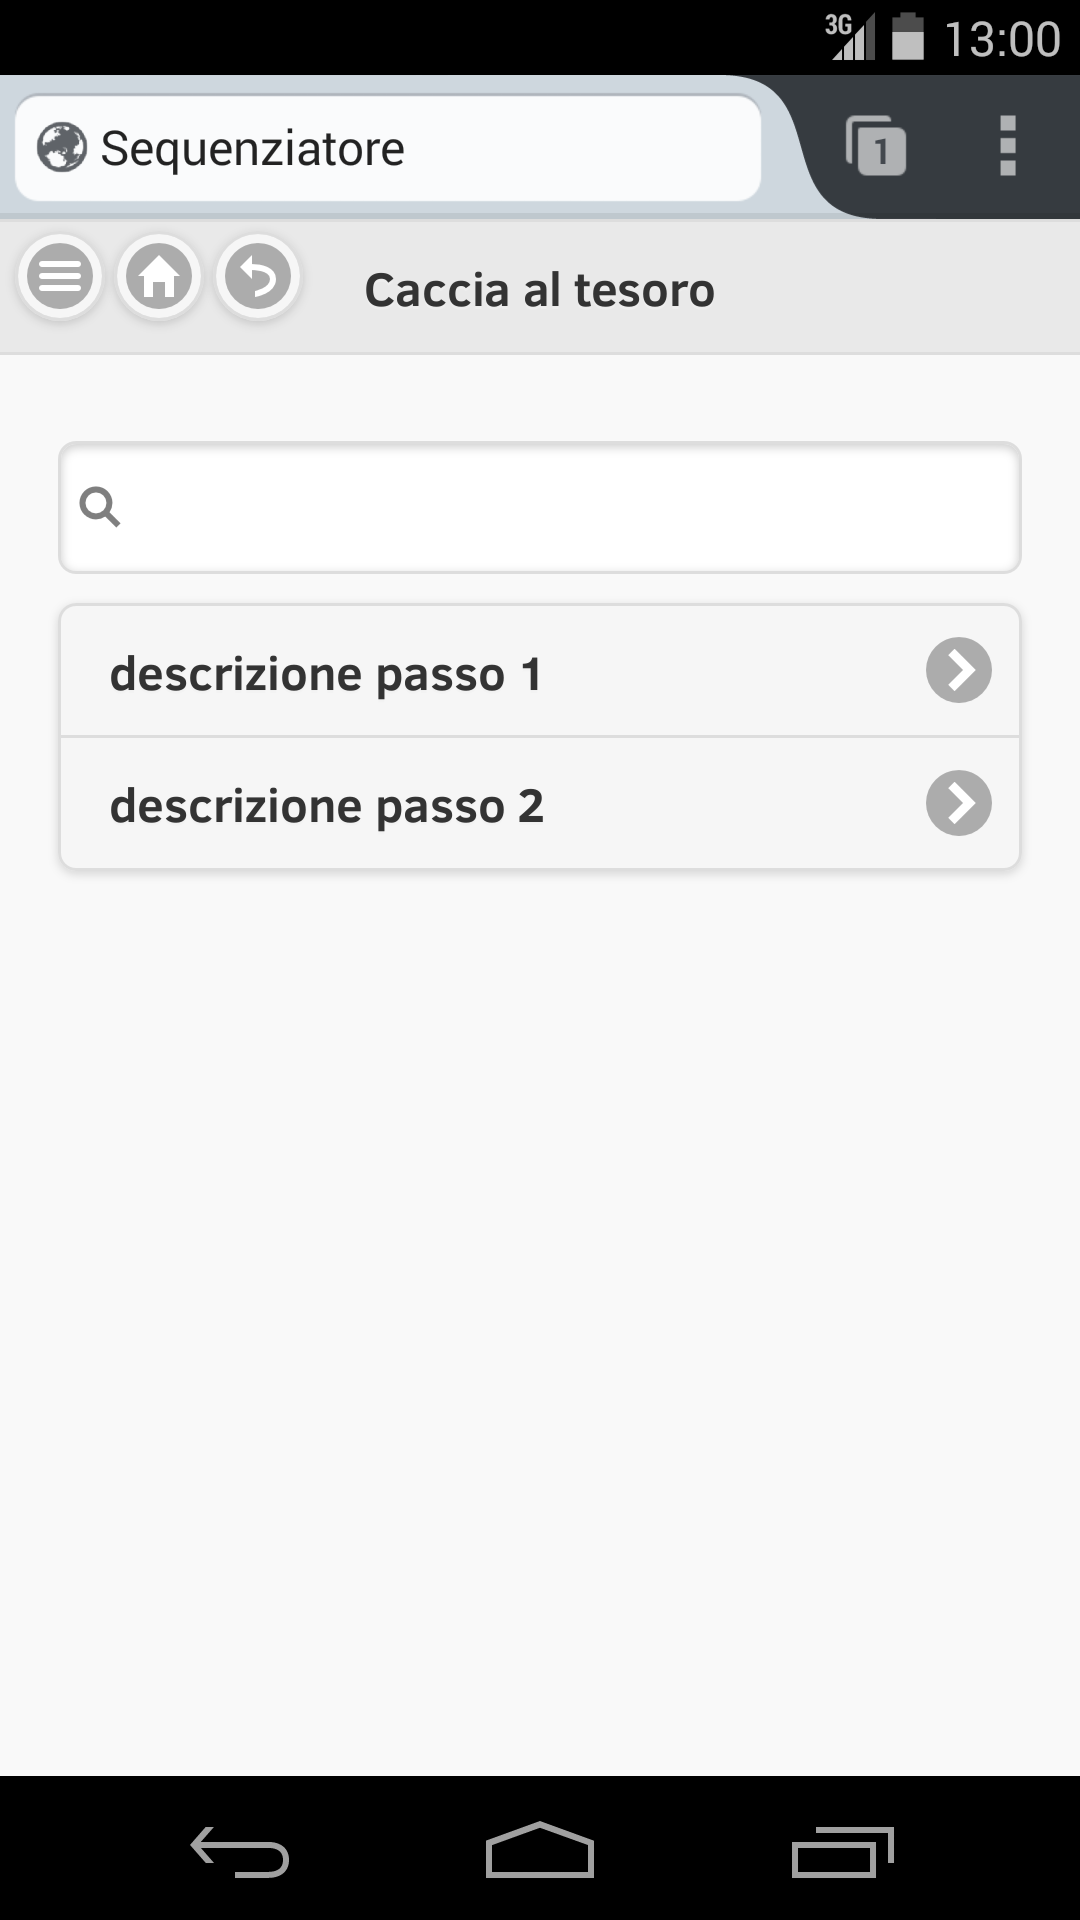
\includegraphics[width=0.5\textwidth]
{./screen/Process.png}} \caption{Gestione del processo selezionato}
\label{fig:Fprocess}
\end{figure}
\fi
In questa pagina è possibile visualizzare la descrizione del processo e scegliere se iscriversi ad esso.
Per iscriversi al processo selezionato è sufficiente premere il pulsante ``Iscriviti''.
Ad iscrizione avvenuta è possibile iniziare le operazioni di \hyperref[gestione]{esecuzione dei processi}.

In altro a sinistra sono presenti i seguenti pulsanti:
\begin{itemize}
\item \textbf{Home:} pulsante che consente di tornare alla \hyperref[home]{pagina principale};
\item \textbf{Opzioni:} apre il pannello laterale in cui è consentita la \hyperref[logout]{chiusura della sessione} e la \hyperref[userdata]{gestione delle credenziali}.;
\item \textbf{Indietro:} pulsante che consente di tornare alla scelta di un processo.
\end{itemize}

\paragraph*{Possibili errori:}
\begin{itemize}
\item \hyperref[e1]{E1}: \textit{javascript\ped{G}} disabilitato;
\item \hyperref[e3]{E3}: errore di connessione al \textit{server\ped{G}}.
\end{itemize}

\subsection{Esecuzione di un processo}
\label{gestione}

\subsubsection{Scelta di un processo}

In figura \hyperref[fig:Fprocesses]{figura \ref{fig:Fprocesses}}, è rappresentata la schermata di gestione dei processi, accessibile dopo aver effettuato l'autenticazione, che consente di selezionare un processo per gestirlo.

\begin{figure}[H] \centering 
\frame{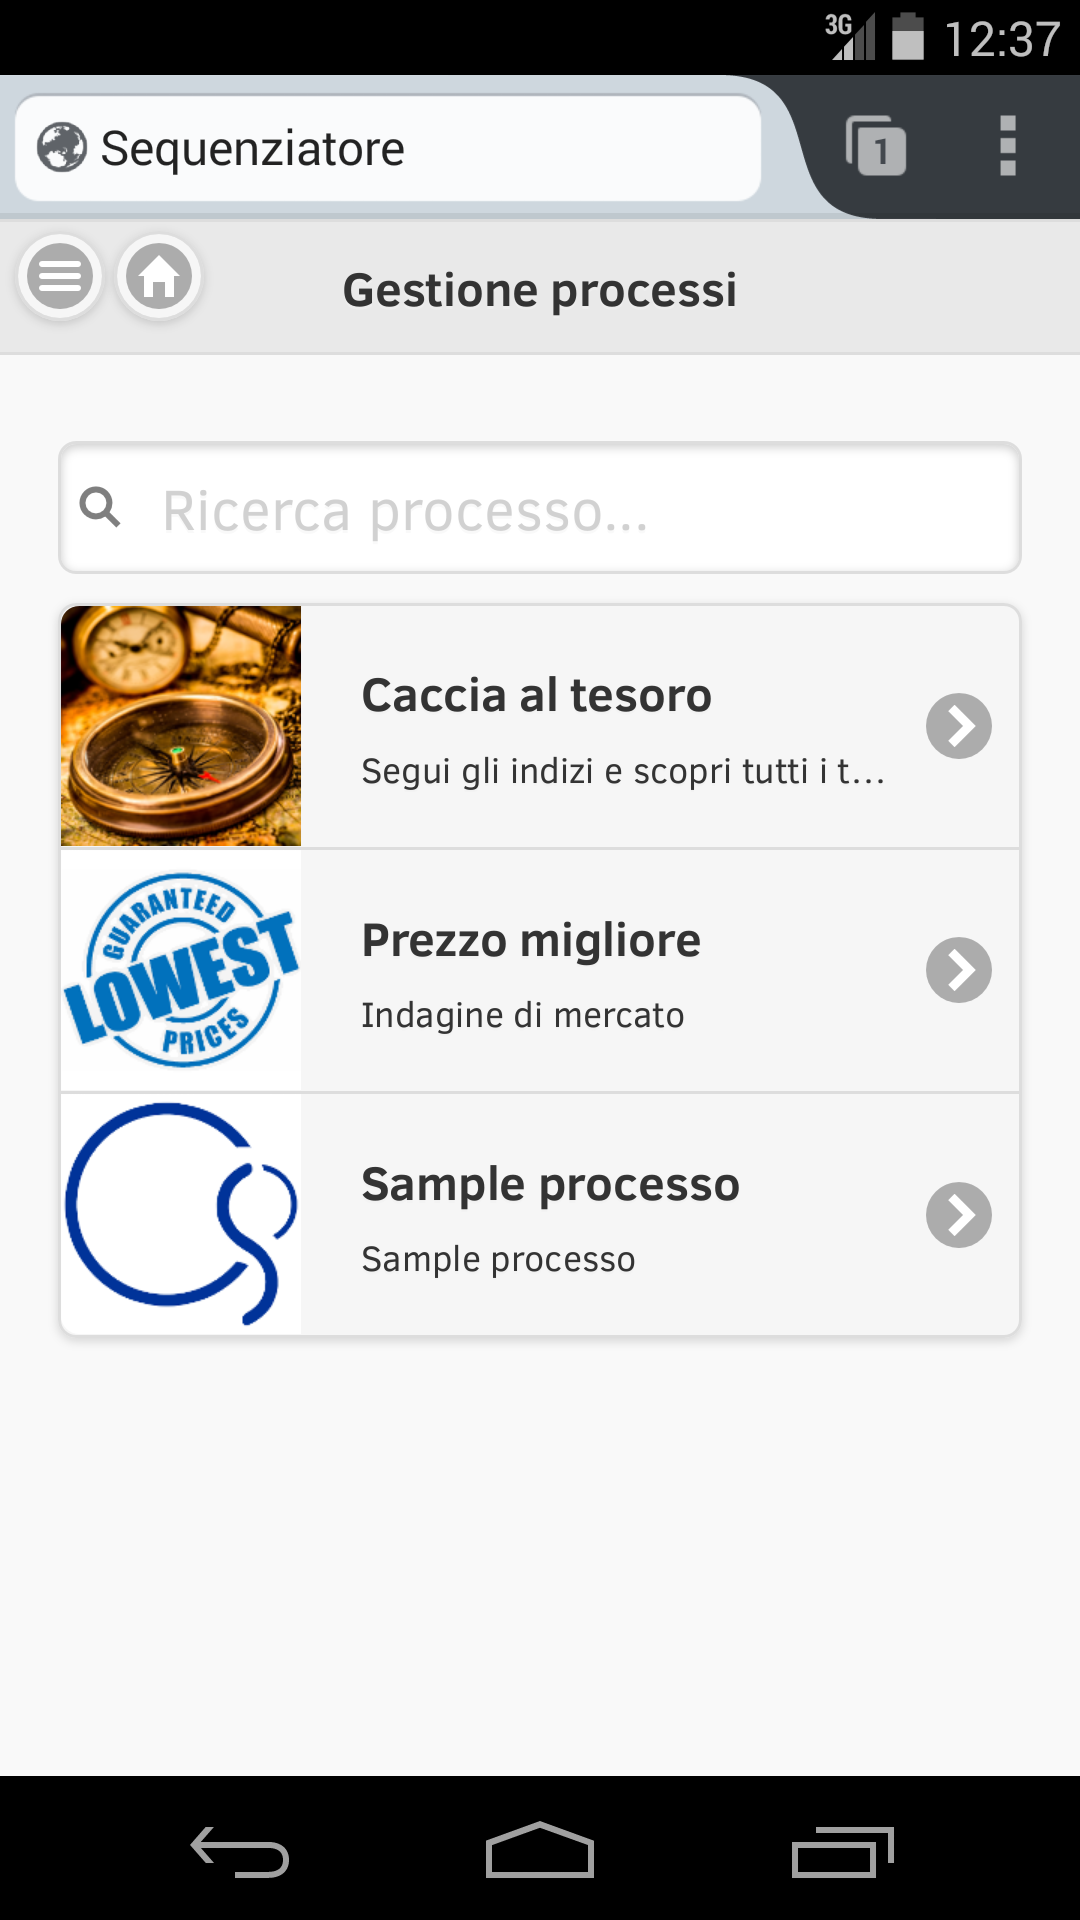
\includegraphics[width=0.5\textwidth]
{./screen/Processes.png}} \caption{Scelta di un processo}
\label{fig:Fprocesses}
\end{figure}

In questa pagina è possibile selezionare uno tra i processi in elenco. È inoltre disponibile la funzionalità di ricerca: inserendo del testo nella barra di ricerca (con suscritto ``Ricerca processo''), l'elenco si aggiornerà, con i soli processi che contengono nel titolo o nella descrizione, il testo oggetto della ricerca.
Per ripristinare l'elenco è sufficiente cancellare il testo nella barra dell'elenco, o premere il pulsante a forma di ``x''.

In altro a sinistra sono presenti i seguenti pulsanti:
\begin{itemize}
\item \textbf{Home:} pulsante che consente di tornare alla \hyperref[home]{pagina principale};
\item \textbf{Opzioni:} apre il pannello laterale in cui è consentita la \hyperref[logout]{chiusura della sessione} e la \hyperref[userdata]{gestione delle credenziali}.
\end{itemize}

\paragraph*{Possibili errori:}
\begin{itemize}
\item \hyperref[e1]{E1}: \textit{javascript\ped{G}} disabilitato;
\item \hyperref[e3]{E3}: errore di connessione al \textit{server\ped{G}}.
\end{itemize}

\subsubsection{Gestione del processo selezionato}

In figura \hyperref[fig:Fprocess]{figura \ref{fig:Fprocess}}, è rappresentata la schermata di gestione del processo selezionato.

\begin{figure}[H] \centering 
\frame{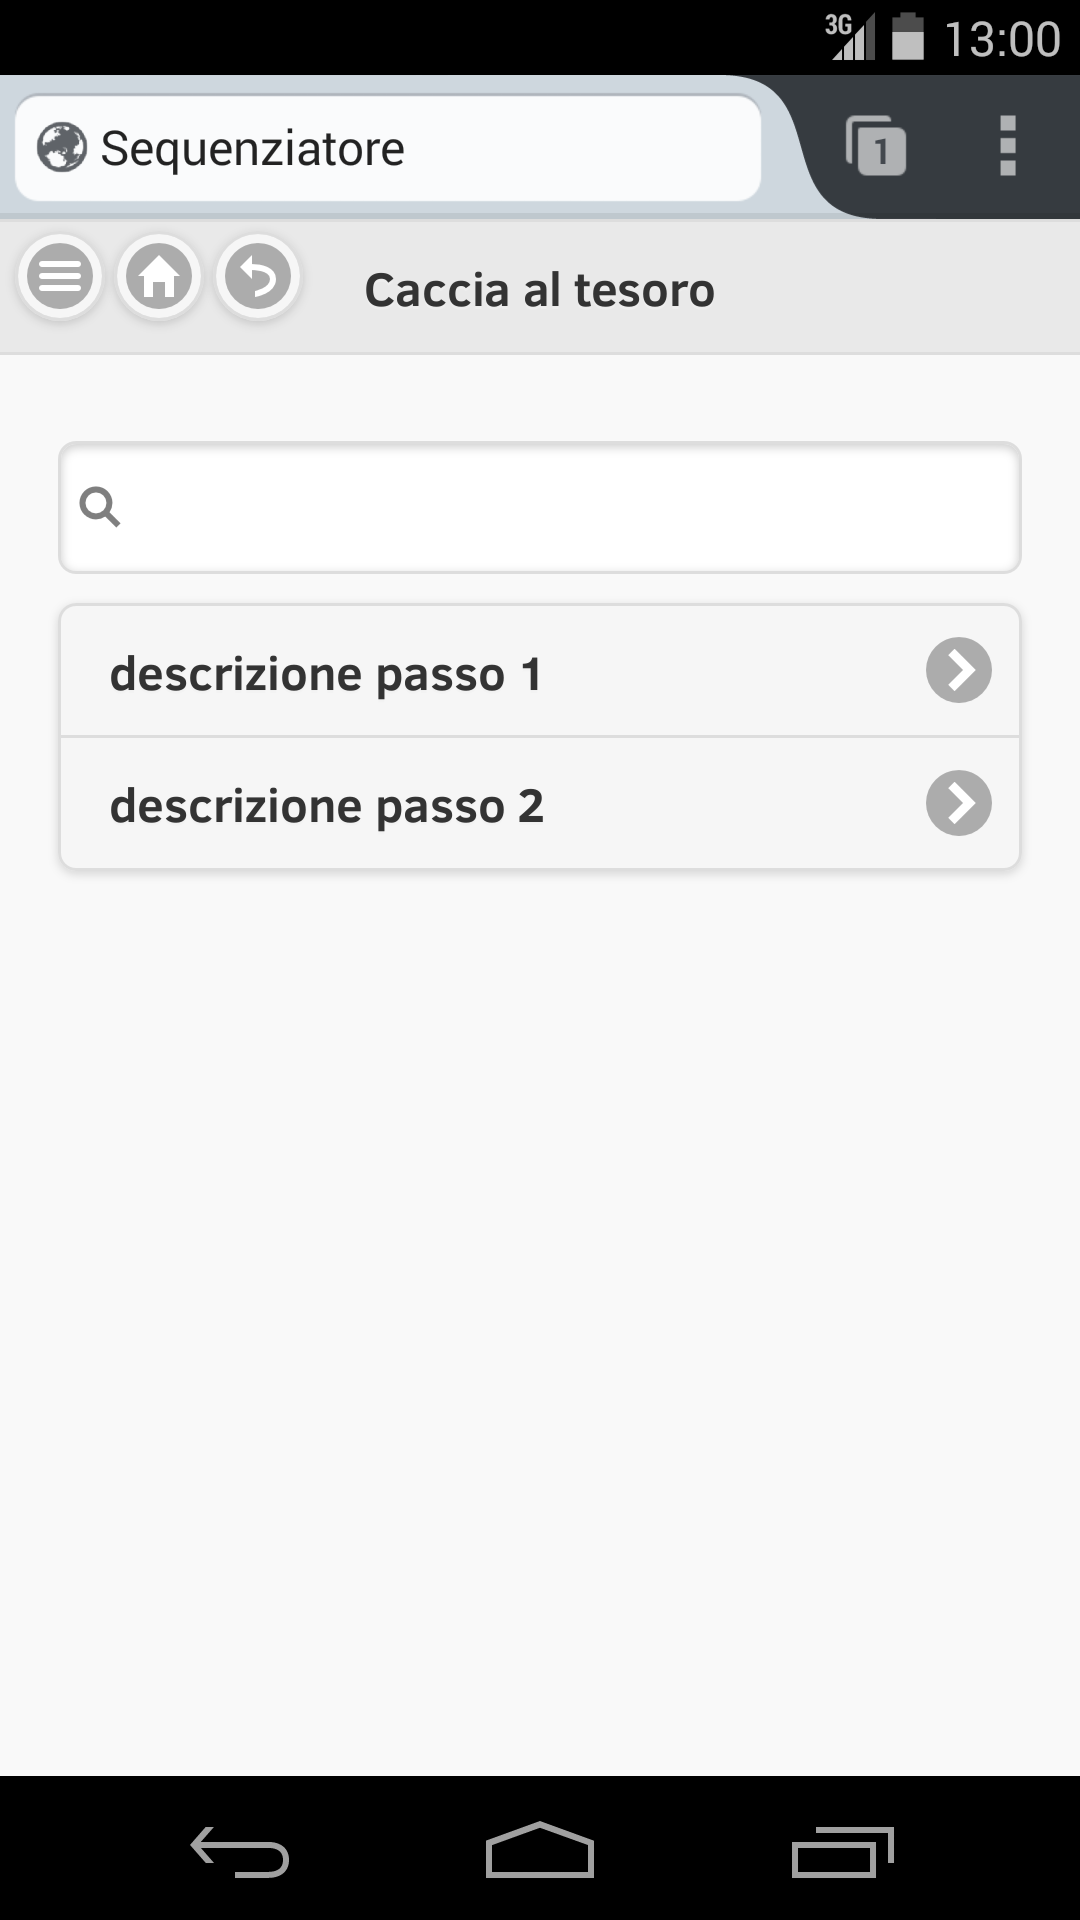
\includegraphics[width=0.5\textwidth]
{./screen/Process.png}} \caption{Gestione del processo selezionato}
\label{fig:Fprocess}
\end{figure}

In questa pagina è possibile visualizzare la descrizione del processo e selezionare uno tra i passi disponibili all'esecuzione. È inoltre disponibile la funzionalità di ricerca: inserendo del testo nella barra di ricerca, l'elenco si aggiornerà, con i soli passi che contengono nella descrizione, il testo oggetto della ricerca.
Per ripristinare l'elenco è sufficiente cancellare il testo nella barra dell'elenco.

In altro a sinistra sono presenti i seguenti pulsanti:
\begin{itemize}
\item \textbf{Home:} pulsante che consente di tornare alla \hyperref[home]{pagina principale};
\item \textbf{Opzioni:} apre il pannello laterale in cui è consentita la \hyperref[logout]{chiusura della sessione} e la \hyperref[userdata]{gestione delle credenziali}.;
\item \textbf{Indietro:} pulsante che consente di tornare alla scelta di un processo.
\end{itemize}

\paragraph*{Possibili errori:}
\begin{itemize}
\item \hyperref[e1]{E1}: \textit{javascript\ped{G}} disabilitato;
\item \hyperref[e3]{E3}: errore di connessione al \textit{server\ped{G}}.
\end{itemize}

\subsubsection{Esecuzione di un passo}
\iffalse
In figura \hyperref[fig:Fexecution]{figura \ref{fig:Fexecution}}, è rappresentata la schermata di esecuzione di un passo, accessibile dopo aver effettuato l'autenticazione.

\begin{figure}[H] \centering 
\frame{\includegraphics[width=0.5\textwidth]
{./screen/Fexecution.png}} \caption{Esecuzione di un passo}
\label{fig:Fstepdata}
\end{figure}
\fi
Questa pagina contiene la descrizione del passo in esecuzione, e la lista dei dati che devono essere inviati dagli utenti per superarlo.

Può essere richiesto l'inserimento di un dato testuale, numerico, o di un immagine.
Per ogni dato richiesto, è importante porre attenzione alla relativa descrizione.
Per inserire un'immagine è sufficiente premere il pulsante ``Aggiungi immagine'' e successivamente su ``Carica immagine'' o ``Scatta foto''.

Per inviare i dati del passo, è sufficiente premere il pulsante ``invia dati''.
I passi facoltativi permettono inoltre di premere il pulsante ``salta passo'', che consente di concludere il passo in esecuzione senza inviare alcun dato.
In altro a sinistra sono presenti i seguenti pulsanti:
\begin{itemize}
\item \textbf{Home:} pulsante che consente di tornare alla \hyperref[home]{pagina principale};
\item \textbf{Opzioni:} apre il pannello laterale in cui è consentita la \hyperref[logout]{chiusura della sessione} e la \hyperref[userdata]{gestione delle credenziali};
\item \textbf{Indietro:} pulsante che consente di tornare alla gestione del processo selezionato.
\end{itemize}

\paragraph*{Possibili errori:}
\begin{itemize}
\item \hyperref[e1]{E1}: \textit{javascript\ped{G}} disabilitato;
\item \hyperref[e3]{E3}: errore di connessione al \textit{server\ped{G}};
\item \hyperref[e5]{E5}: dato mancante;
\item \hyperref[e8]{E8}: vincolo non rispettato.
\end{itemize}

\subsection{Chiusura della sessione}
\label{logout}
In figura \hyperref[fig:Flogout]{figura \ref{fig:Flogout}}, è rappresentato il pannello laterale, visualizzabile premendo il pulsante opzioni (vedi pulsante in alto a sinistra in \hyperref[fig:Fhome]{figura \ref{fig:Fhome}}), da qualsiasi pagina accessibile dopo aver effettuato l'autenticazione.

\begin{figure}[H] \centering 
\frame{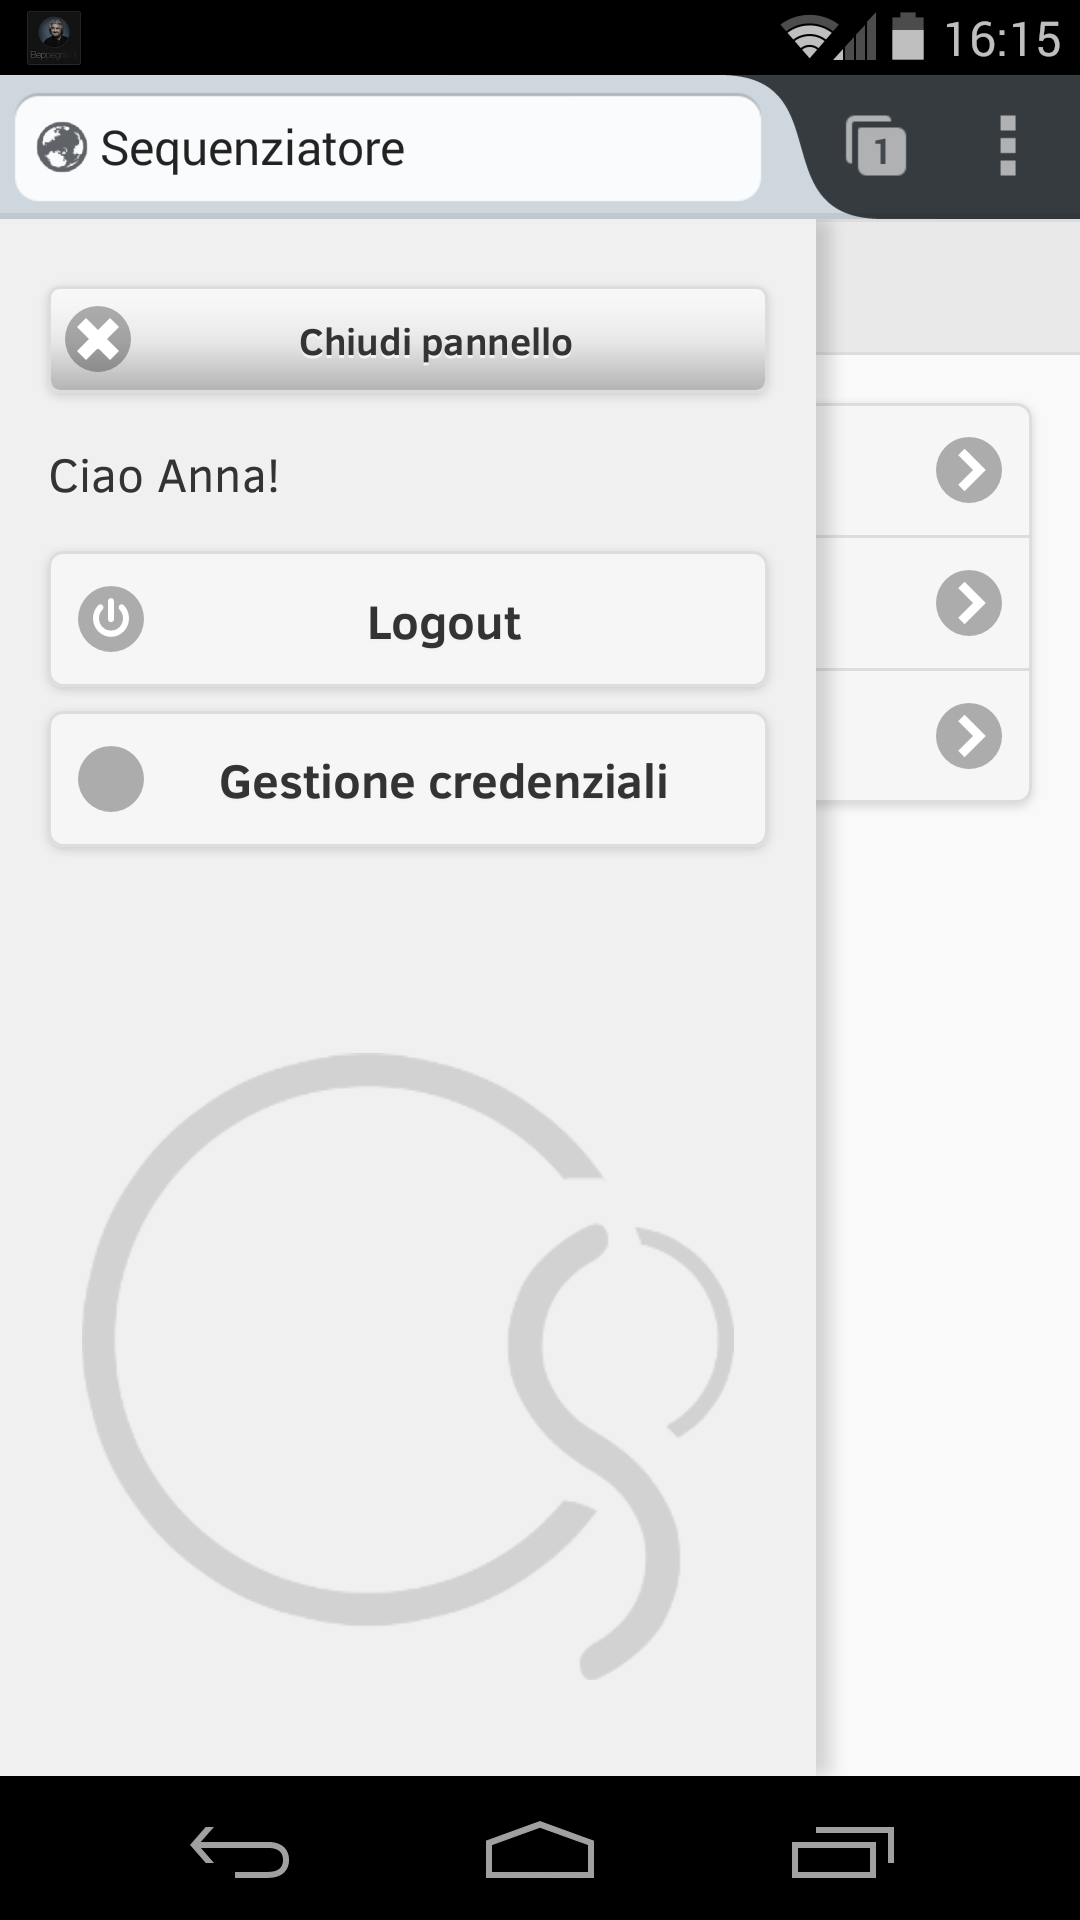
\includegraphics[width=0.5\textwidth]
{./screen/Logout.png}} \caption{Pannello laterale}
\label{fig:Flogout}
\end{figure}

Premendo il pulsante ``chiudi pannello'' è possibile ritornare alla pagina da cui il pannello è stato aperto.
Premendo il pulsante ``Logout'' l'utente ritornerà alla pagina di \hyperref[autenticazione]{autenticazione}, e i suoi dati di sessione\ped{G} vengono eliminati.

\subsubsection*{Possibili errori:}
\begin{itemize}
\item \hyperref[e1]{E1}: \textit{javascript\ped{G}} disabilitato.
\end{itemize}